\begin{figure*}[t]
    \centering
    % \fbox{\rule{0pt}{2in} \rule{1.0\linewidth}{0pt}}
    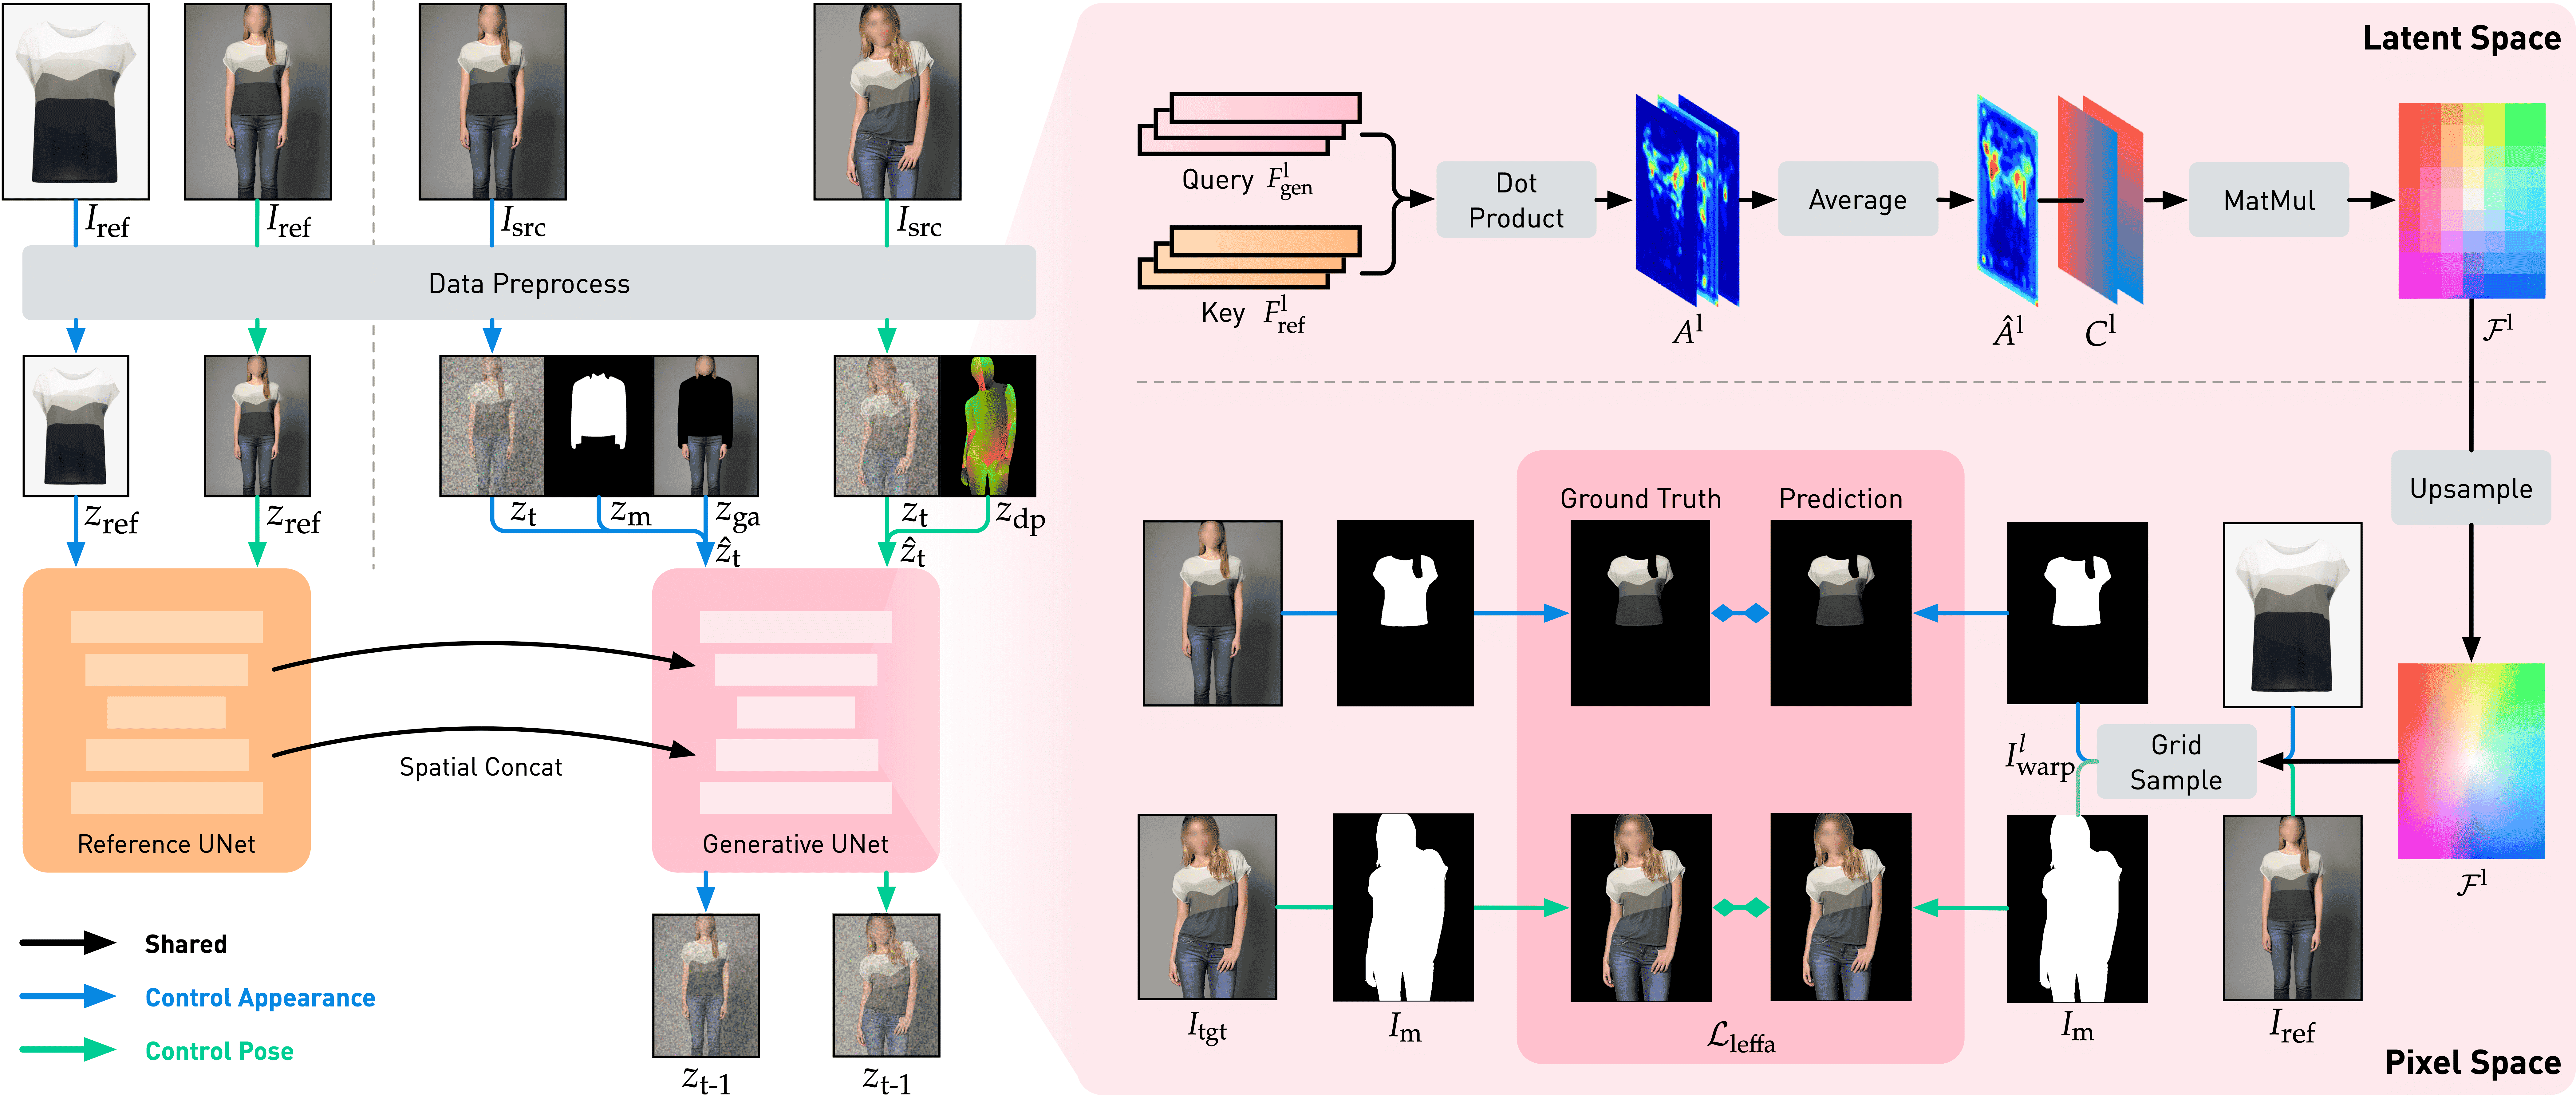
\includegraphics[width=1.0\linewidth]{Chapter6/Figures/leffa_final-min.png}
    \caption{An overview of our \leffa{} training pipeline for controllable person image generation.
    The left is our diffusion-based baseline; the right is our \leffa{} loss.
    Note that $I_\text{src}$ and $I_\text{tgt}$ are the same image during training.
    }
    \label{leffa:fig:overview}
\end{figure*}


\section{Preliminary}
\label{leffa:sec:preliminary}

\subsection{Diffusion Model}

Diffusion models~\citep{ho2020denoising, rombach2022high} have gained popularity in image generation models due to their stable training and exceptional generative capabilities.
Among them, the Stable Diffusion (SD) series (\eg, SD1.5~\citep{rombach2022high}, SDXL~\citep{podell2023sdxl}) is widely used.
SD is a latent diffusion model (LDM), consisting of a variational autoencoder (VAE)~\citep{kingma2013auto}, a UNet~\citep{ronneberger2015u} $\epsilon_{\theta}(\cdot)$, and text encoders~\citep{raffel2020exploring, radford2021learning}.
The VAE includes an encoder $\mathcal{E}(\cdot)$ and a decoder $\mathcal{D}(\cdot)$, which encodes input images from a pixel space into a latent space to reduce computational cost.
During training, we first use the encoder $\mathcal{E}(\cdot)$ of VAE to encode a given image into a latent feature $\mathbf{z}_\text{0}$.
At a sampled diffusion time step $t \in \{1, \cdots, T\}$, we apply a Gaussian noise $\epsilon \sim \mathcal{N}(0, 1)$ to the latent feature $\mathbf{z}_\text{0}$ based on a noise scheduler, obtaining a noised latent feature $\textbf{z}_t$.
The UNet $\epsilon_{\theta}(\cdot)$ then denoises the noised latent feature $\textbf{z}_t$ under the control of the conditional feature $\textbf{c}$.
Formally, the training loss can be formulated as:
\begin{equation}
    \mathcal{L}_{\text{diffusion}} = \mathbb{E}_{\epsilon \sim \mathcal{N}(0,1),t} [ \| \epsilon - \epsilon_{\theta}(\textbf{z}_t, \textbf{c}, t) \|_{2}^{2} ],
\label{eq:loss_diffusion}
\end{equation}
where $\textbf{c}$ can be either the language feature predicted by the text encoders or the visual feature derived from the reference image, which is the primary focus of our work.


\subsection{Task Definition and Notations}

\noindent Given a source person image $I_{\text{src}} \in \mathbb{R}^{H \times W \times 3}$ and a reference image $I_{\text{ref}} \in \mathbb{R}^{H \times W \times 3}$, controllable person image generation aims to generate a target person image $I_{\text{tgt}} \in \mathbb{R}^{H \times W \times 3}$, where $H$ and $W$ denote the height and width of the image.
Specifically, in virtual try-on, $I_{\text{tgt}}$ represents the garment image $I_{\text{ref}}$ worn on the person in $I_{\text{src}}$; while in pose transfer, $I_{\text{tgt}}$ represents the person in $I_{\text{ref}}$ adopting the pose from $I_{\text{src}}$.
During training, $I_{\text{src}}$ and $I_{\text{tgt}}$ are the same image.
The data preprocessing for each task is defined as follows:

\begin{itemize}
    \item For virtual try-on, following~\cite{choi2024improving, chong2024catvton}, we first extract a garment mask $I_\text{m} \in \{0, 1\}^{H \times W \times 1}$ from $I_\text{src}$ and construct a garment-agnostic image $I_\text{ga} \in \mathbb{R}^{H \times W \times 3} = I_\text{src} * (1 - I_\text{m})$.
    During training, we encode $I_\text{src}$ and $I_\text{ga}$ via the VAE encoder $\mathcal{E}(\cdot)$ yields $z_\text{0}$ and $z_\text{ga}$, and resize $I_\text{m}$ to latent space as $z_\text{m}$.
    We add noise to $z_\text{0}$ based on the sampled time step $t$ which produces $z_t$, and we channel concatenate it with $z_\text{ga}$ and $z_\text{m}$ to construct $\hat{z_t}$.
    \item For pose transfer, following~\cite{han2023controllable}, we first extract a DensePose image~\citep{guler2018densepose} $I_\text{dp} \in \mathbb{R}^{H \times W \times 3}$ from $I_\text{src}$.
    During training, we encode $I_\text{src}$ with the VAE encoder $\mathcal{E}(\cdot)$, obtaining $z_\text{0}$, and resize the $I_\text{dp}$ to the latent resolution of $z_\text{dp}$.
    We add noise to $z_\text{0}$ at sampled time step $t$ to produce $z_t$, and we channel concatenate it with $z_\text{dp}$ to construct $\hat{z_t}$.
\end{itemize}
For the reference image $I_{\text{ref}}$ in both tasks, we encode it into a latent feature $z_{\text{ref}}$, and use that as a conditional feature within a diffusion loss defined in Eq.~\ref{eq:loss_diffusion}.


\section{Method}
\label{leffa:sec:method}

Our goal is to leverage diffusion-based methods to preserve fine-grained details while maintaining high overall image quality.
To achieve this, we propose the \leffa{} loss that alleviates detail distortion through learning flow fields in attention.
To validate the effectiveness of \leffa{}, we first construct a unified diffusion-based baseline suitable for both virtual try-on and pose transfer tasks in Sec.~\ref{leffa:sec:baseline}.
We then introduce the formulation of \leffa{} loss in Sec.~\ref{leffa:sec:leffa}.
Lastly, we explain its integration into the model training in Sec.~\ref{leffa:sec:training}.

\subsection{Diffusion-based Baseline}
\label{leffa:sec:baseline}

We first design our diffusion-based baseline upon the SD~\citep{rombach2022high, podell2023sdxl} to assess the effectiveness of our \leffa{} loss.
Specifically, we modify SD in two steps as follows.

First, we duplicate the pre-trained SD UNet $\epsilon_{\theta}(\cdot)$ to create two separate UNets: i) a Generative UNet $\epsilon_{\theta_{\text{gen}}}(\cdot)$ for processing $\hat{z_t}$ from the source image $I_\text{src}$; and ii) a Reference UNet $\epsilon_{\theta_{\text{ref}}}(\cdot)$ for processing $z_\text{ref}$ from the reference image $I_\text{ref}$.
Since we only condition on images, we remove both the text encoders and the cross-attention layers used for text interaction in the Generative UNet $\epsilon_{\theta_{\text{gen}}}(\cdot)$ and Reference UNet $\epsilon_{\theta_{\text{ref}}}(\cdot)$.
Notably, both UNets are \textit{fully trainable}, which we found to be effective in our early exploration.

Second, to condition the generation of the target person image $I_{\text{tgt}}$ on $I_{\text{src}}$ and $I_{\text{ref}}$, we employ \textit{spatial concatenated} self-attention.
For $l$-th attention layer, we define the generative features fed into the Generative UNet $\epsilon_{\theta_{\text{gen}}}(\cdot)$ as $F_{\text{gen}}^{l} \in \mathbb{R}^{n^{l} \times d^{l}}$, and the reference features in the Reference UNet $\epsilon_{\theta_{\text{ref}}}(\cdot)$ as $F_{\text{ref}}^{l} \in \mathbb{R}^{n^{l} \times d^{l}}$, where $n^{l} = h^{l} \times w^{l}$ with $h^{l}$ and $w^{l}$ as spatial dimensions, and $d^{l}$ as the feature dimension.
We concatenate the $F_{\text{ref}}^{l}$ with $F_{\text{gen}}^{l}$ along the spatial dimension, yielding concatenated feature $F_{\text{cat}}^{l} \in \mathbb{R}^{2n^{l} \times d^{l}}$, and jointly feed it into the Generative UNet's self-attention layer.
We retain only the first half of the output corresponding to $F_{\text{gen}}^{l}$ for further processing.
This process is repeated across all self-attention layers.

Using SD's training method and the loss function in Eq.~\ref{eq:loss_diffusion}, our clean and simple diffusion-based baseline already achieves performance comparable to current state-of-the-arts~\citep{kim2024stableviton, choi2024improving, chong2024catvton, wan2024improving, bhunia2023person, han2023controllable, lu2024coarse, pham2024cross}, while relying on no additional auxliary models (\eg, CLIP~\citep{radford2021learning}, DINOv2~\citep{oquab2023dinov2}) and/or complicated training techniques (\eg, DREAM~\citep{zhou2024dream}).
However, this diffusion-based baseline still suffers from detail distortion, which will be addressed by the \leffa{} loss, introduced in the next section.


\subsection{\textbf{\leffa{}}: Learning Flow Fields in Attention}
\label{leffa:sec:leffa}

Our goal is to preserve fine-grained details without textural distortion.
Detail distortion arises when the target query in the attention layer fails to attend to the corresponding region of the reference key correctly.
To address this, we propose the \leffa{} loss, which explicitly guides the target query to \textit{spatially focus} on the correct region of the reference key through supervision by learning flow fields in attention.

Specifically, in the $l^{th}$ attention layer of the Generative UNet $\epsilon_{\theta_{\text{gen}}}(\cdot)$, we compute the attention map $A^{l}$ by using $F_{\text{gen}}^{l}$ as the query $Q$ and $F_{\text{ref}}^{l}$ as the key $K$, formulated as the dot-product attention defined in \cite{vaswani2017attention},
\begin{equation}
    A^{l} = \texttt{softmax} \bigg( \frac{Q K^{\top}}{\sqrt{d}} / \tau \bigg),
\end{equation}
where $\tau$ is the temperature coefficient, and $d$ is the token size of the query $Q$.
We then construct the \leffa{} loss based on the attention map $A^{l}$.

For each attention map $A^{l}$, we aim to encourage all query tokens in $F_{\text{gen}}^{l}$ to attend to the correct regions on the reference key $F_{\text{ref}}^{l}$.
Following \citet{darcet2023vision}, we also include additional learnable tokens to allow flexible attention on other regions.
This design, rather than enforcing strict spatial attention alignment in all attention heads, we ensure that, \textit{on average}, attention maps across different heads focus on the correct region.
To achieve this, we average $A^{l}$ across the head dimension, resulting in $\hat{A^{l}} \in \mathbb{R}^{n^{l} \times n^{l}}$.

Next, we convert $\hat{A^{l}}$ to a flow field representing the spatial correspondence between $I_\text{src}$ and $I_\text{ref}$.
To achieve this, we construct a normalized coordinate map $C^{l} \in \mathbb{R}^{n^{l} \times 2}$, where, reshaped as $\mathbb{R}^{h^{l} \times w^{l} \times 2}$, within the top-left coordinate $(0, 0)$ has the value of $[-1, -1]$ and the bottom-right coordinate $(h-1, w-1)$ has the value of $[1, 1]$.
We then multiply the attention map $\hat{A^{l}}$ with the coordinate map $C^{l}$ to obtain the flow field $\mathcal{F}^{l} \in \mathbb{R}^{n^{l} \times 2}$, formulated as
\begin{equation}
    \mathcal{F}^{l} = \hat{A^{l}} \cdot C^{l},
\end{equation}
which indicates the coordinates of the region on the reference feature $F_{\text{ref}}^{l}$ that each target query token attends to.

We then use this flow field $\mathcal{F}^{l}$ as a coordinate mapping and apply the grid sampling operation to warp the reference image $I_{\text{ref}}$ into the target image $I_{\text{tgt}}$.
Considering our method is based on the latent diffusion model, the resolution of the attention map is significantly lower than the original input image.
To provide precise pixel-level training supervision, we upsample the flow field in $l^{th}$ attention layer $\mathcal{F}^{l}\in\mathbb{R}^{h^{l} \times w^{l} \times 2}$ to the original image resolution using bilinear interpolation, resulting in the upsampled flow field $\mathcal{F}_{up}^{l} \in \mathbb{R}^{H \times W \times 2}$.
We then use this upsampled flow field $\mathcal{F}_{up}^{l}$ to warp the reference image $I_{\text{ref}}$, producing the warped image ${I_{\text{warp}}^{l}} \in \mathbb{R}^{H \times W \times 3}$.

Finally, we compute the L2 loss between ${I_{\text{warp}}^{l}}$ and the corresponding region of the target image $I_{\text{tgt}}$, which defines our \leffa{} loss formulation:
\begin{equation}
     \mathcal{L}_{\text{leffa}} = \sum\nolimits_{l=1}^{L}  \Vert I_{\text{tgt}} * I_m - {I_{\text{warp}}^{l}} * I_m \Vert_{2}^{2}.
\end{equation}
This loss supervises the attention map without additional inputs or parameters, ensuring each target query token attends to the correct reference region and preserving fine-grained detail consistency in the generated images.

Note that, we apply \leffa{} loss only on selected $L$ attention layers, explained next.


\subsection{Model Training with \textbf{\leffa{}} Loss}
\label{leffa:sec:training}
In this section, we detail the application of \leffa{} loss to the diffusion-based baseline, guiding the target query to attend to the correct reference key and thus alleviating fine-grained detail distortion.

We follow \citet{zhu2024m} to adopt progressive training with \leffa{} loss, applied in the final finetuning phase to avoid early-stage performance degradation.
The model is initially trained at a low resolution (\eg, $256$, $512$), then at a higher resolution (\eg, $1024$).
In the final phase, we fine-tune at $1024$ resolution using a combined loss:
\begin{equation}
    \mathcal{L}_{\text{finetune}} = \mathcal{L}_{\text{diffusion}} + \lambda_\text{leffa} \mathcal{L}_{\text{leffa}},
\end{equation}
where $\lambda_\text{leffa}$ is the loss weight of $\mathcal{L}_{\text{leffa}}$.
For optimal model performance with \leffa{} loss, we also address the following considerations.

\noindent \textbf{Attention Layer Selection.}
Given that current LDM-based methods perform feature interaction between the target and reference images in the latent space, the resulting attention maps tend to have relatively low resolution.
For such low-resolution attention maps, accurately warping the reference image $I_{\text{ref}}$ is not feasible.
Therefore, we set a resolution threshold $\theta_{\text{resolution}} = h/H$ (\eg, $1/32$), representing the ratio of the attention map size to the original image size (see Fig.~\ref{leffa:fig:ablation}).
Only attention layers with a resolution greater than $\theta_{\text{resolution}}$ participate in the computation of $\mathcal{L}_{\text{leffa}}$.

\noindent \textbf{Timestep Selection.}
When the time step $t$ is large, substantial noise is added to the image, making accurate feature interactions between the target and reference difficult due to the excessive noise, which hinders attending to the right semantics of the corresponding regions.
Therefore, \leffa{} loss is not suitable for large time steps (see Fig.~\ref{leffa:fig:ablation}).
We thereby set a timestep threshold $\theta_{\text{timestep}}$ (\eg, $500$ when $T=1000$), and during training, only time steps smaller than $\theta_{\text{timestep}}$ are included in the calculation of $\mathcal{L}_{\text{leffa}}$.

\noindent \textbf{Temperature Selection.}
Different temperatures adjust the smoothness of the attention map produced by softmax.
A larger temperature results in a smoother attention map, allowing the target query token to attend to a broader range of reference features $F_{\text{ref}}^{l}$, which helps the model more easily learn the correct reference regions and increases tolerance to errors (see Fig.~\ref{leffa:fig:ablation}).
Therefore, when using \leffa{} loss, we apply a relatively large temperature $\tau$ (\ie, 2.0).
